\graphicspath{{introduction/fig/}}

\chapter{Introduction}
\label{chap:introduction}

\begin{quote}
    "We don't tell [computers] what to do, we give them examples... The problem is, sometimes we don't understand how it figured it out."\\ % <--- FORCED NEW LINE HERE
    \vspace{0.5em} % Adds a slightly larger vertical space after the quote text
    \hfill -- Jeff Dean, Head of Google AI \cite{Dean2017BlackBox}
\end{quote}


The prevalence of neural networks (NNs) has positioned them as a foundational technology in modern artificial intelligence. However, as their use has grown, so too has the focus on their inherent mechanistic limitations. Two of the most significant drawbacks of NNs are their lack of explainability---the "black-box" effect---and the immense computational cost required for training. A novel field, weight space learning, emerges as an field showing promise to further our understanding of these very challenges.

Weight space learning primarily focuses on developing methods to represent the high-dimensional, weights of NN models in a lower-dimensional latent space, in order to facilitate further exploration of the weight space. The field generally considers two types of tasks: discriminative and generative.

In the discriminative application, models use the weights of already-trained models, with a specific collection of models reffered to as a model zoo, as input to accurately predict meta-information about the original model. The quality of weight space representation is often quantitatively measured by a simple Multi-layer perceptron (MLP)'s ability to predict this meta-information, conditioned only on the model's weight space representation. 

Common meta-information metrics investigated include predicting the model's final performance and the generalization gap (the difference between training and validation loss). For instance, the Sequential Autoencoder for Neural Embeddings (SANE) \cite{schurholt2024scalableversatileweightspace} demonstrated strong performance in meta-prediction tasks. Furthermore, research has shown that weight embeddings can encode fundamental training characteristics, such as accurately recovering the size of the dataset on which the model was originally trained \cite{salama2024datasetsizerecoverylora}. These discriminative tasks serve the dual purpose of both validating the quality of the derived weight representations and possessing significant practical value.

In the generative application, researchers leverage the structure of the latent weight space to create new, functional models. For example, \cite{schurholt2024scalableversatileweightspace} (SANE) makes use of an autoencoder for sequentially encoding and decoding models, with a bottleneck layer generating the latent vector, and then a decoder to generate a full model. Another paper uses a Vector Quantized Variational Autoencoder (VQ-VAE), which takes in information about the dataset as part of the process of find latent weight representations, with the ultimate going of instruction-guided paramter generation \cite{bedionita2025instructionguidedautoregressiveneuralnetwork}.\cite{meynent2025structureenoughleveragingbehavior} makes use of information on the model's performance and behavior in generating the model embeddings. With $P(W \mid \dots)$ being the distribution sampled from to generate new model weights, currently no existing paper conditions on both dataset information $(\mathcal{D})$ and model performance $(R)$ simultaneously, modeling the conditional distribution:

$$ 
 P(W \mid \mathcal{D} , R)
$$

Problem Statement: To what extent can we develop contrastive methods to project model input and model predictive performance to a latent weight space, thereby accurately modeling the complex relationship between a model's weights, its inputs, and its resulting behavior?
% TODO {introduction}

The focus of this report is to develop a extend latent weight representations into a shared, multimodal representation space. Figure \ref{fig:pipeline} outlines this proposed pipeline.

\begin{figure}[!t]
    \centering
    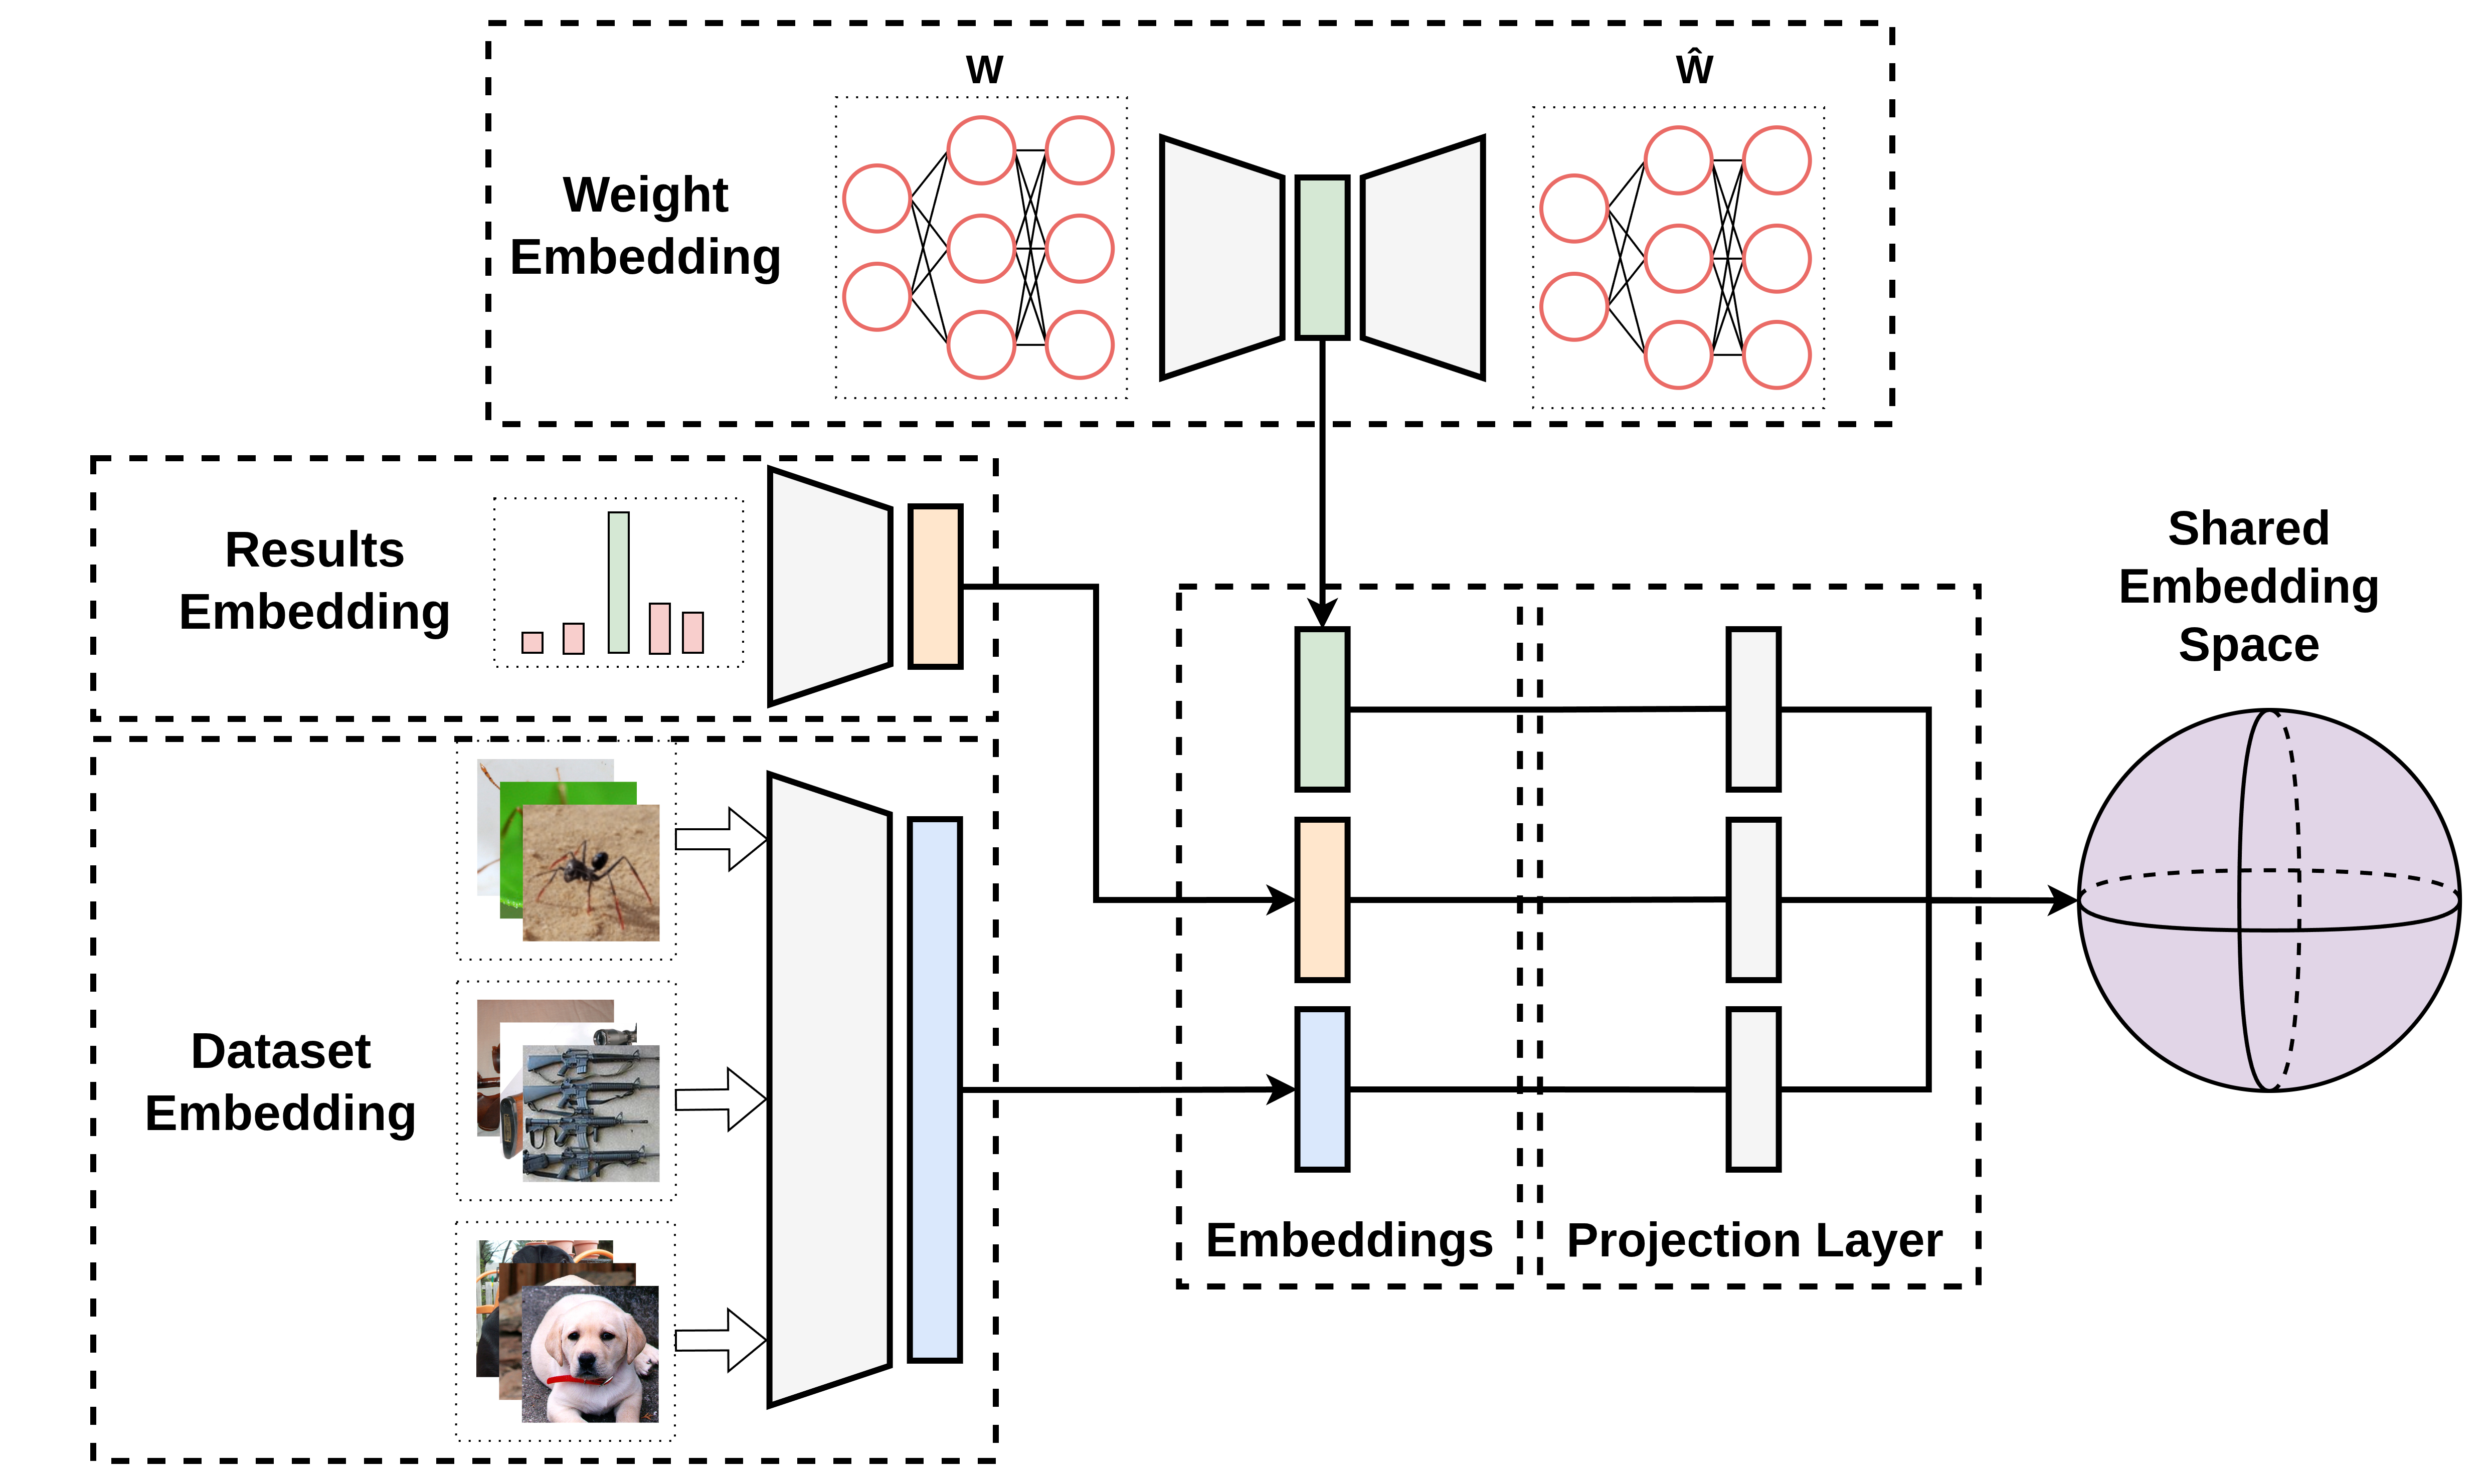
\includegraphics[width=0.75\linewidth]{pipeline.png}
    \caption[A figure illustrating the process of embedding a dataset,model weigths and results into a shared embedding space ]{A representation of the process of embedding a dataset, model weights and results in a shared embedding space. A dataset embedded using a pretrained CLIP encoder, averaging over all images. Model weights embedded using a PCA enhanced autoregressive encoder. Model results embeddings and the shared embedding space created through contrastive learning   }
    \label{fig:pipeline}
\end{figure}

The results found from the report, and how it's limited 

The remainder of this report is structured as follows.:

    % TODO {outline_paragraph}
    In Section 1 we will discuss x, next y, concluded by z in attempt to showcase that this report is the best
    % TODO {outline_paragraph}

% TODO {introduction}






% \section{Section heading}

% This is some section with two table in it: Table~\ref{tbl:exemplars} and Table~\ref{tbl:abx_speaker}.

% \begin{table}[!h]
%     \mytable
%     \caption{Performance of the unconstrained segmental Bayesian model on TIDigits1 over iterations in which the reference set is refined.}
%     \begin{tabularx}{\linewidth}{@{}lCCCCC@{}}
%         \toprule
%         Metric     & 1 & 2 & 3 & 4 & 5 \\
%         \midrule
%         WER (\%)                        & $35.4$ & $23.5$ & $21.5$ & $21.2$ & $22.9$ \\
%         Average cluster purity (\%)       & $86.5$ & $89.7$ & $89.2$ & $88.5$ & $86.6$ \\
%         Word boundary $F$-score (\%)         & $70.6$ & $72.2$ & $71.8$ & $70.9$ & $69.4$ \\
%         Clusters covering 90\% of data   & 20             & 13 & 13 & 13 & 13 \\
%         \bottomrule
%     \end{tabularx}
%     \label{tbl:exemplars}
% \end{table}


% \begin{table}[!h]
%     \renewcommand{\arraystretch}{1.1}
%     \centering
%     \caption{A table with an example of using multiple columns.}
%     \begin{tabularx}{0.65\linewidth}{@{}lCCr@{}}
%         \toprule
%         & \multicolumn{2}{c}{Accuracy (\%)} \\
%         \cmidrule(lr){2-3}
%         Model    & Intermediate & Output & Bitrate\\
%         \midrule
%         Baseline & 27.5         & 26.4   & 116 \\
%         VQ-VAE   & 26.0         & 22.1   & 190 \\
%         CatVAE   & 28.7         & 24.3   & 215 \\
%         \bottomrule
%     \end{tabularx}
%     \label{tbl:abx_speaker}
% \end{table}

% \newpage

% This is a new page, showing what the page headings looks like, and showing how to refer to a figure like Figure~\ref{fig:cae_siamese}.

% \begin{figure}[!t]
%     \centering
% %     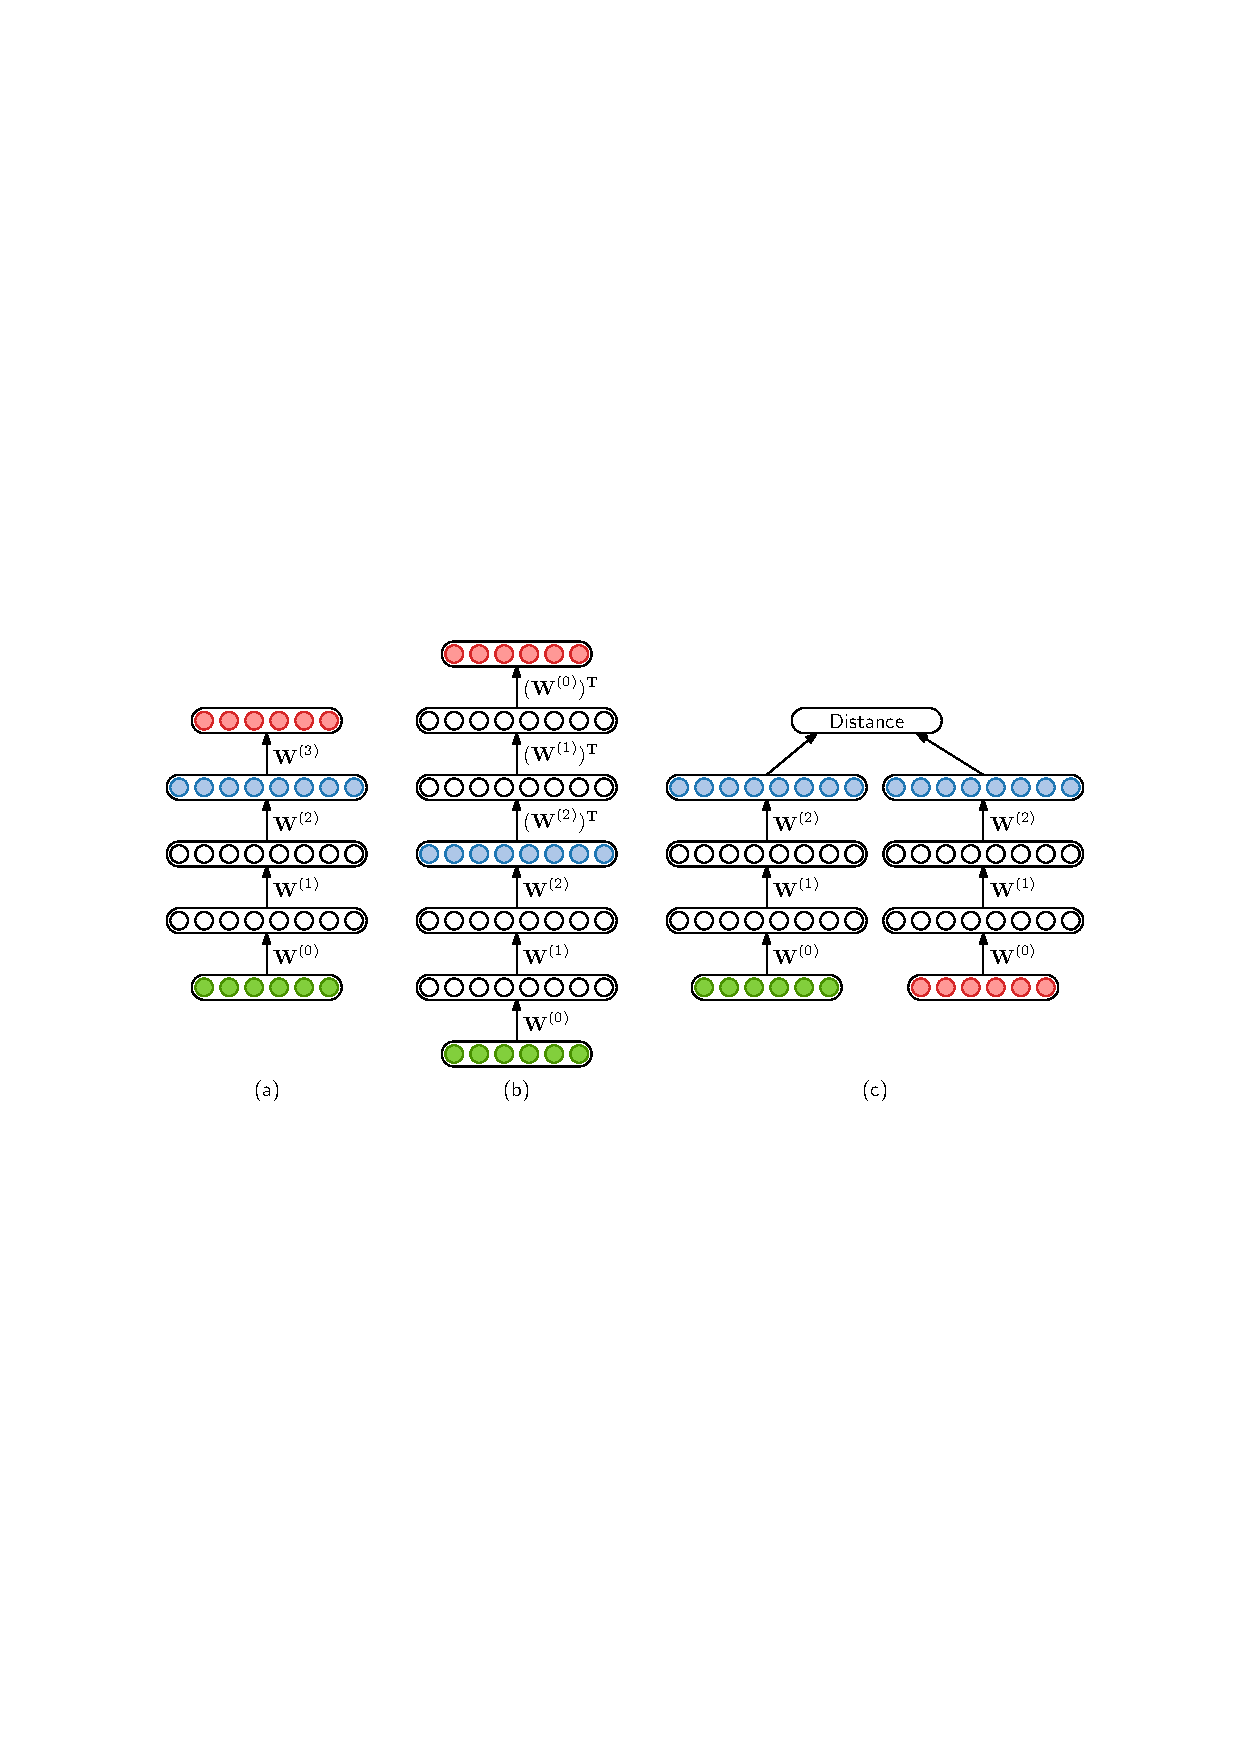
\includegraphics[width=\linewidth]{cae_siamese}
%     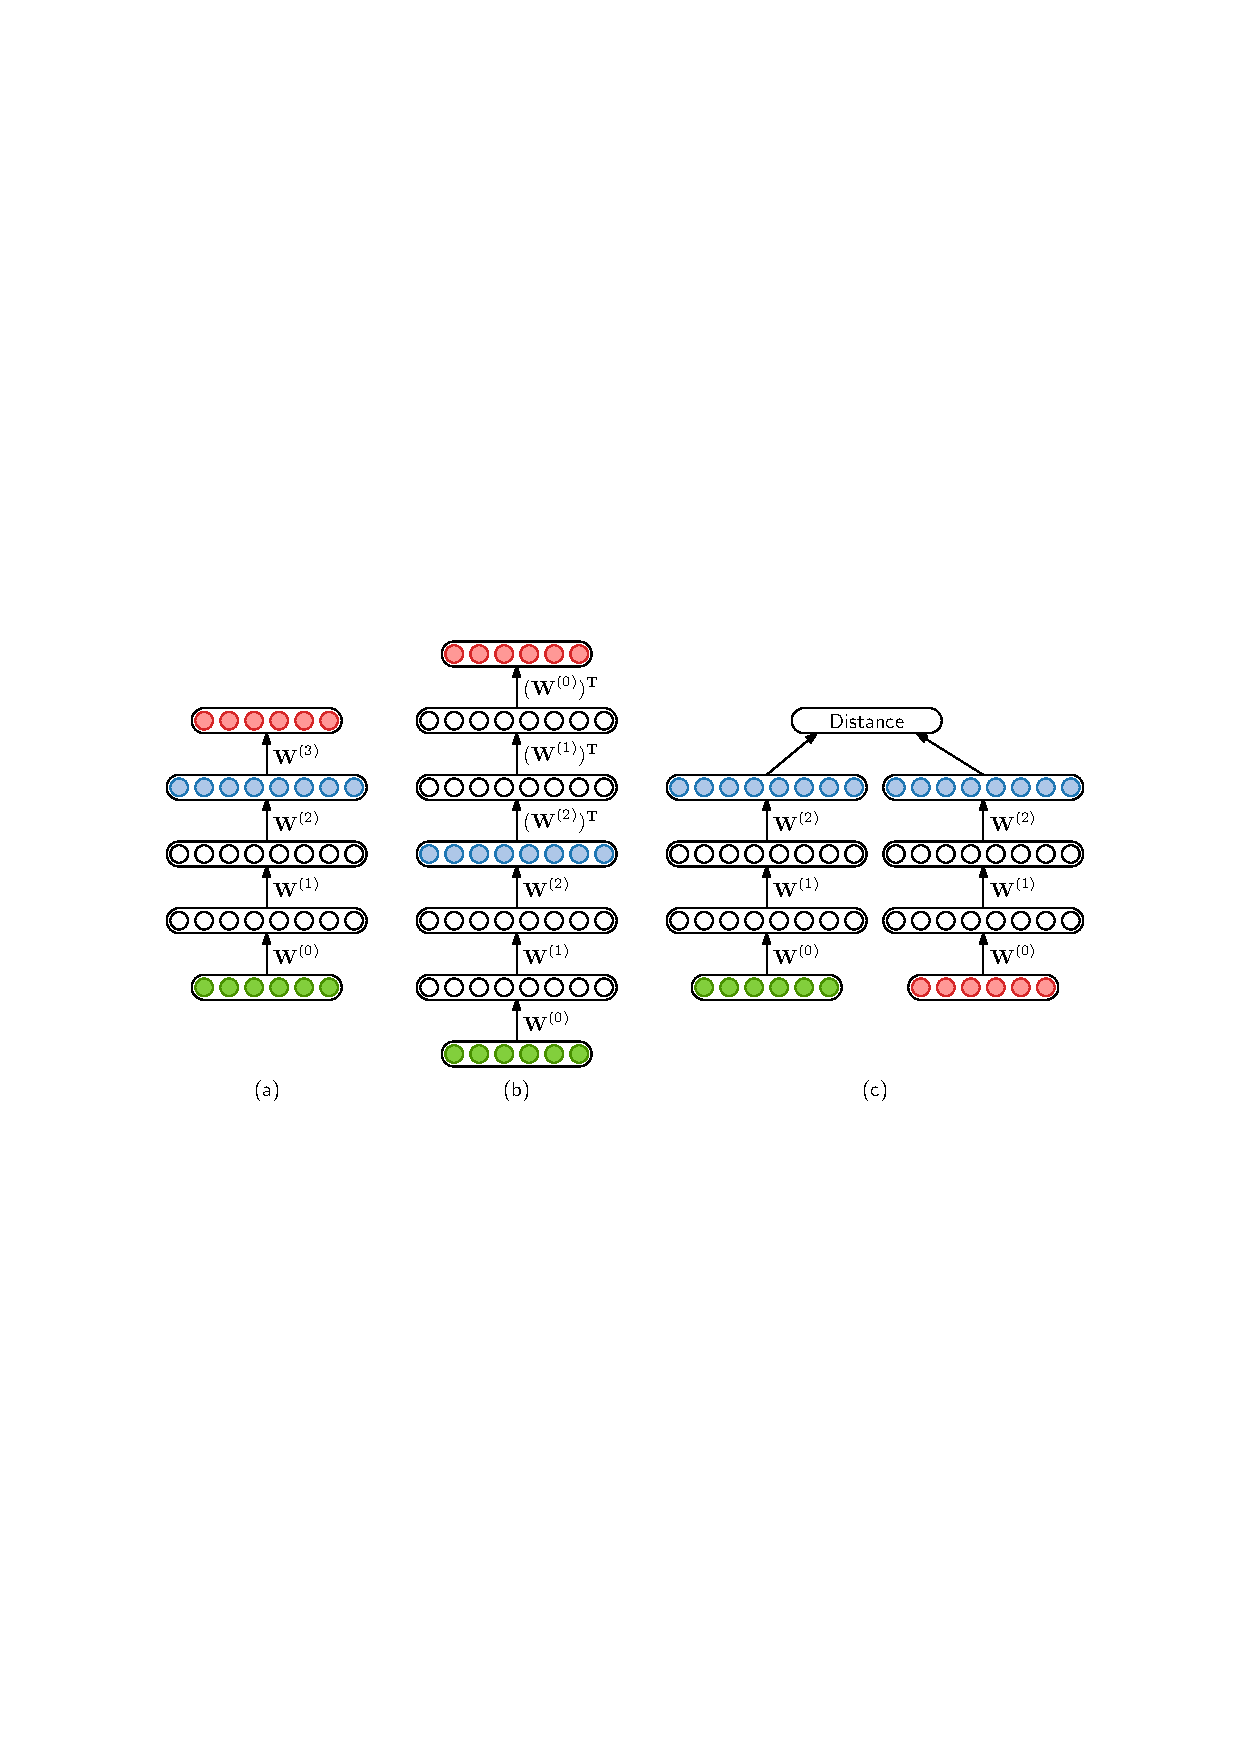
\includegraphics[width=0.918\linewidth]{cae_siamese}
%     \caption[I am the short caption that appears in the list of figures, without references.]{
%     (a) The cAE as used in this chapter. The encoding layer (blue) is chosen based on performance on a development set.
%     (b) The cAE with symmetrical tied weights. The encoding from the middle layer (blue) is always used.
%     (c) The siamese DNN. The cosine distance between aligned frames (green and red) is either minimized or maximized depending on whether the frames belong to the same (discovered) word or not.
%     A cAE can be seen as a type of DNN~\cite{dahl+etal_taslp12}.
%     }
%     \label{fig:cae_siamese}
% \end{figure}


% The following is an example of an equation:
% \begin{equation}
% P(\vec{z} | \vec{\alpha}) = \int_{\vec{\pi}} P(\vec{z} | \vec{\pi}) \, p(\vec{\pi} | \vec{\alpha}) \, \textrm{d} \vec{\pi}
% = \int_{\vec{\pi}} \prod_{k = 1}^K \pi_k^{N_k} \frac{1}{B(\vec{\alpha})} \prod_{k = 1}^K \pi_k^{\alpha_k - 1} \, \textrm{d} \vec{\pi}
% \label{eq:example_equation}
% \end{equation}
% which you can subsequently refer to as~\eqref{eq:example_equation} or Equation~\ref{eq:example_equation}.
% But make sure to consistently use the one or the other (and not mix the two ways of referring to equations).


